\section{Implementation and Evaluation}
\label{sec:dyadic-count-sketch-implementation}

In order to facilitate easy implementation in a wide range of languages, including those from the functional programming paradigm, the operations of the dyadic count sketch are presented in the pseudocode as free-standing functions that operate on immutable input data structures without side effects.
The Java implementation takes full advantage of the object-oriented programming paradigm, however, and the corresponding methods are instance members of the mutable \lstinline{DyadicCountSketch} class, which implements the \lstinline{getRank(int)} and \lstinline{getItem(int)} query methods of the \lstinline{RankSummary} and \lstinline{QuantileSummary} interfaces, respectively.
This class implements the extended version of the summary described in \cref{subsec:dyadic-count-sketch-analysis-universe}, which adapts the original definition of the sketch to accept items from an extended universe of both positive and negative items.
For this reason, the universe of items used in the implementation is defined to be a subset of the full range of the ubiquitous \num{32}~bit signed \lstinline{int} data type.
This allowed the implementation to use the same item data type as that of the \lstinline{Fingerprint} and the \lstinline{CountSketch} (see \cref{sec:fingerprint-implementation,sec:count-sketch-implementation}).
For a similar reason, the \lstinline{int} data type is also used to represent weights.
This means that the update methods of the \lstinline{Fingerprint}, the \lstinline{CountSketch} and the \lstinline{DyadicCountSketch} can share the signature \lstinline{update(int, int)}, which is declared in the \lstinline{MultisetSummary} interface.

Since the universe of the \lstinline{int} data type is a dyadic interval of size \( 2^{32} \), the dyadic structure has \num{32}~levels.
Each level maintains a frequency summary that can be queried for an approximation of the frequency of all items that appear in a given dyadic interval of the universe (see \cref{sec:dyadic-count-sketch-theory}).
The number of lower levels is calculated using the number of rows and the number of columns passed to the \lstinline{DyadicCountSketch(int, int)} constructor.
Each lower level summarizes the data using a \lstinline{CountSketch}, whose implementation is described in \cref{sec:count-sketch-implementation}.
Each upper level instead stores exact frequencies using a \lstinline{FrequencyTable}, which is a static implementation of the \lstinline{FrequencySummary} interface nested within \lstinline{DyadicCountSketch}.
This class maintains a frequency table as an array and stores the exact frequency of an item in the position that corresponds to its value.
Since each reduced domain of the universe has a negative lower bound, an offset is applied to shift each item to a non-negative index.
Since both the \lstinline{CountSketch} and the \lstinline{FrequencyTable} classes implement the \lstinline{FrequencySummary} interface, the dyadic structure can be stored as an array of \num{32} \lstinline{FrequencySummary} objects.
This allows calls to the update, merge and query methods of each level to be resolved using polymorphism, which provides an optimization over the definitions of the operations given in \cref{sec:dyadic-count-sketch-theory}, as it removes the need for conditional checks and branching in order to treat the upper and lower levels accordingly~\citep{dasu02}.
Due to the relationship between dyadic intervals and the binary number system, the dyadic interval to which the item is mapped on each level~\( l \) is given by the two's complement interpretation of the first \( 32 - l \) bits of the item.
Thus, it could be considered more semantically accurate for items to be mapped to intervals in the levels above and below the current level via signed right shift and left shift, respectively, rather than the floor division and multiplication by two presented in \cref{alg:dyadic-count-sketch-theory-rank-query,alg:dyadic-count-sketch-theory-quantile-query,alg:dyadic-count-sketch-analysis-universe-extended-quantile-query}.
For this reason, the bit shift operations are preferred in the implementation.
Taken on their own, machine language instructions for bit shift operations are almost always more efficient than those of multiplication and division, although, in practice, modern compilers can usually optimize multiplication and division to a series of bit shifts and addition~\citep{warren12}.
This is particularly trivial for multiplication and division by powers of two.

The \lstinline{DyadicCountSketchAccumulator} class adapts the summary for use in Apache Spark (see \cref{subsec:introduction-structure-library}).
This allowed two types of test to be performed on the implementation of the dyadic count sketch.
The first was a test of the accuracy of its query operation.
The second was a test of the relationship between the size of a dataset and the time taken to construct its summary.
All tests were performed on a single machine using an Intel Core i5-9300H CPU with a base clock speed of \SI{2.40}{\giga\hertz}, four physical cores and eight logical processors, and \SI{8}{\gibi\byte} of RAM\@.
For information regarding how to run the tests, see \cref{app:repository}.

A failure in the accuracy of a dyadic count sketch occurs when the absolute error in its approximation of the rank of an item exceeds an error bound expressed as a fraction of the cardinality \( \cardinality{S} \) of the multiset it summarizes.
This error bound is given in \cref{subsec:dyadic-count-sketch-analysis-accuracy}.
This states that a dyadic count sketch whose constituent count sketches each have \( m = \lg (\lg (u) / \varepsilon) \) rows and \( n = (1 / \varepsilon) \cdot \sqrt{\lg (u) \cdot \lg (\lg (u) / \varepsilon)} \) columns gives estimates whose absolute errors are at most \( \varepsilon \cdot \cardinality{S} \) with constant probability.
This can be verified empirically by varying the upper bound of the interval from which the weights are drawn.

Five series of accuracy tests were performed using the upper bounds \( 2^{4} - 1 \), \( 2^{6} - 1 \), \( 2^{8} - 1 \), \( 2^{10} - 1 \), and~\( 2^{12} - 1 \).
Since the accuracy guarantee only holds if the multiplicity of every item is non-negative when the sketch is queried, a fixed lower bound of zero was used in all tests.
To obtain a representative sample of results, each test was run \num{25}~times.
On each run, an artificial dataset was generated by drawing \( 2^{16} \) pairs of items and weights uniformly at random from the universe of items and the interval of weights, respectively.
This dataset size was chosen as it is large enough to warrant the use of a streaming algorithm, which offers a reduction in space requirements in exchange for less accurate results.
Conversely, it is not so large that the time and space consumed by the test could prevent other tests from being performed.
For a similar reason, a total of \( 2^{16} \) queries were performed on the dyadic count sketch constructed from each dataset.
The items chosen to be queried were distributed uniformly over the universe from which items were drawn.
This was the reason for the choice of upper bounds.
The greatest upper bound \( 2^{12} - 1 \) is small enough that in the unlikely case that all \( 2^{16} \)~items in the dataset are the same, and that their weights are all the upper bound \( 2^{12} - 1 \), the \num{32}-bit signed integer data type used to represent multiplicities in the implementation will not overflow.
Since the accuracy is independent of the size of the universe of items, the items were drawn from the full range of the \num{32}-bit signed integer data type used to represent items in the implementation.

To save time and space, a small number of rows was chosen.
An odd number of rows allows each constituent count sketch to return the true median of the estimates of each item.
Since the implementation uses \( \lg (u) = 32 \), the smallest odd number of rows that results in an error bound less than \SI{100}{\percent} of the cardinality of the multiset is seven.
This corresponds to an error bound of \SI{25}{\percent} of the cardinality of the multiset, and a width of \num{60}~columns.

Using the Apache~Spark stream processing framework, each dataset was read as input and passed one pair at a time to a \lstinline{DyadicCountSketchAccumulator}, which constructed a \lstinline{DyadicCountSketch} of the multiset.
Apache~Spark was run using one worker thread for each of the eight logical processors of the test machine.
By running the summary construction in parallel, the correctness of the merge operation was also verified.
The summary was queried for approximations of the ranks of \( 2^{16} \) items.
Each approximation was compared to the corresponding true rank in the dataset, and its absolute error was calculated.
If this exceeded the error bound \( \varepsilon \cdot \cardinality{S} \), the query was considered to have failed.
If any query of any run of any test failed, the entire series of tests was considered to have failed.

\begin{table}
  \centering
  \caption{Results of the accuracy tests}
  \label{tab:dyadic-count-sketch-implementation-accuracy}
  \begin{tabular}{
  S[
    table-alignment = right,
    table-format = 4,
  ]
  S[
    table-alignment = right,
    table-format = 1,
  ]
}
  \toprule
  {Weight upper bound} & {Failures} \\
  \midrule
  16 & 0 \\
  64 & 0 \\
  256 & 0 \\
  1024 & 0 \\
  4096 & 0 \\
  \bottomrule
\end{tabular}
%
\end{table}

The results of all \num{25}~runs of each of the five accuracy tests are presented in \cref{tab:dyadic-count-sketch-implementation-accuracy}.
This includes the weight upper bound and the number of failures observed.
Every query passed on every run of every test.
This provides an empirical verification of the correctness of both the design of the extended version of the dyadic count sketch, and the upper bound on the probability of an error.
It should be noted that it is impossible to prove empirically that an approximation will never exceed the error bound.
Nevertheless, the total of \num{125}~runs was sufficient to show that the probability of a failure is low.

The relationship between the size of a dataset and the time taken to construct its summary was tested via performance tests.
Five series of performance tests were performed using dataset sizes of \( 2^{8} \), \( 2^{12} \), \( 2^{16} \), \( 2^{20} \) and~\( 2^{24} \).
For each of the five series, \num{26}~artificial datasets were generated by drawing the corresponding numbers of pairs of items and weights, in the same manner as for the accuracy tests.
Since only the size of the data was varied for these tests, the items were drawn from the full range of the \num{32}-bit signed integer data type, and the weights were drawn from the fixed non-negative interval \( \dataintegerinterval{0, 2^{7} - 1} \).
After all \num{26}~datasets had been generated, the construction of the \lstinline{DyadicCountSketch} of each dataset was timed using only a single worker thread.
The execution time was calculated as the positive difference between the values returned by calls to \lstinline{System.nanoTime()} immediately before and immediately after the construction.
Although this method gives nanosecond precision by querying the most precise available system timer~\citep{o14}, it does not necessarily give nanosecond accuracy, since there is no guarantee regarding the frequency with which this value is updated~\citep{lambert08}.
Nevertheless, it can be assumed that, on average, it is accurate to within hundreds of nanoseconds~\citep{kuperberg09}.
The first run of each series of tests was discarded, as this run `warms up' the test architecture by loading process data into memory and, therefore, encounters page faults and cache misses that should not be considered a feature of normal operation~\citep{luo04}.
The median of the remaining \num{25}~runs was calculated.
Since the execution time can vary greatly due to the presence of other processes, the median is more suitable than the mean as a representation of the typical execution time, as it is not so easily skewed by outliers, and remains meaningful after normalization~\citep{fleming86}.
A sixth series of tests was performed using a dataset containing only a single item--weight pair.
The median execution time of this series was taken as an approximation of the fixed overhead associated with starting the test and initializing the summary.
This was subtracted from the median execution times of the other series of tests in order to normalize them such that they represent only the time taken to update the summary for each item--weight pair in the corresponding dataset.

\begin{table}
  \centering
  \caption{Results of the performance tests}
  \label{tab:dyadic-count-sketch-implementation-performance}
  \begin{tabular}{
  S[
    table-alignment = right,
    table-format = 8,
  ]
  S[
    table-alignment = right,
    table-format = 11,
  ]
  S[
    table-alignment = right,
    table-format = 11,
  ]
}
  \toprule
  {Dataset size} & \multicolumn{2}{c}{Execution time / \si{\nano\second}} \\
  \cmidrule{2-3}
  & {Median} & {Normalized} \\
  \midrule
  1 & 23927624 & 0 \\
  256 & 23971901 & 44277 \\
  4096 & 24566401 & 638777 \\
  65536 & 72955400 & 49027776 \\
  1048576 & 767910300 & 743982676 \\
  16777216 & 13115900199 & 13091972575 \\
  \bottomrule
\end{tabular}
%
\end{table}

\begin{figure}
  \centering
  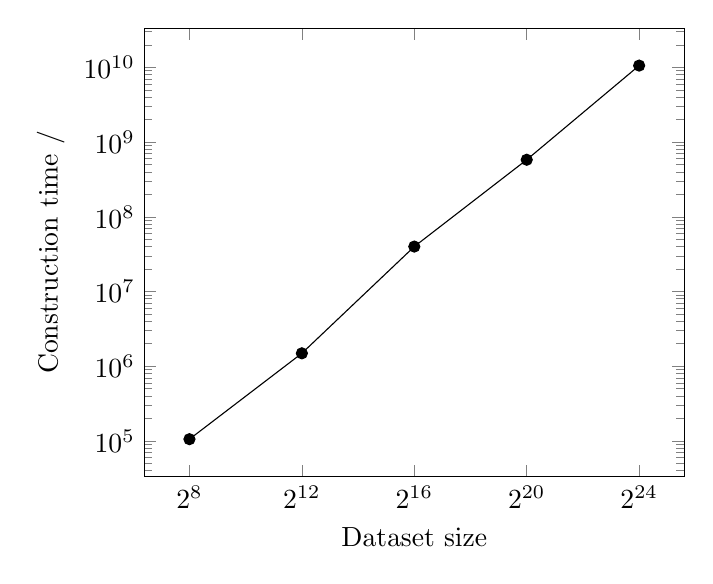
\begin{tikzpicture}
  \begin{loglogaxis}[
    log basis x = 2,
    log basis y = 10,
    xlabel = {Dataset size},
    xtick = {2^8, 2^12, 2^16, 2^20, 2^24},
    ylabel = {\text{Construction time} / \si{\nano\second}},
  ]
    \addplot [mark=*,black] coordinates {
      (256, 105790)
      (4096, 1490690)
      (65536, 39960390)
      (1048576, 579476090)
      (16777216, 10547981289)
    };
  \end{loglogaxis}
\end{tikzpicture}
%
  \caption{Relationship between dataset size and summary construction time}
  \label{fig:dyadic-count-sketch-implementation-performance}
\end{figure}

The results of all \num{25}~runs of each of the five performance tests are presented in \cref{tab:dyadic-count-sketch-implementation-performance}, and the relationship between the size of a dataset and the time taken to construct its summary is shown in \cref{fig:dyadic-count-sketch-implementation-performance}.
This relationship appears to be linear, which agrees with the analysis given in \cref{subsec:dyadic-count-sketch-analysis-complexity}.
Since the update operation has constant time complexity per update in the size of the data---not to be confused with its time complexity \( \bigo{\lg (u) \cdot m} \) in the size \( u \) of the universe and the number of rows \( m \)---and one update is performed for every item--weight pair in the dataset, the time complexity associated with performing all the updates given in a dataset is linear in the size of the dataset.
